%!TEX root = ../main.tex
\section{Board Design} % (fold)
\label{sec:board_design}
Multiple electronics components are required to realise the double pendulum being developed throughout this report.
This section explores the design of those components and the communication between them.
Most of the circuitry is combined on a single PCB, the driver board, however some of the functionality is moved to smaller boards, local to the place where they are needed.\\

The components of the system are listed here:
\begin{itemize}
	\item Motor Encoder
	\item Joint Encoder
	\item End Stops
	\item Motor Driver
	\item Emergency Circuitry
	\item Relay Driver
	\item RF Transceiver
	\item MicroZed 
\end{itemize}
Many of these components require a number of subcomponents, which will be explored further in later sections.

\subsection{Voltage Rails} % (fold)
\label{sub:voltage_rails}
In the design of the board it is necessary to determine which voltage rails are required for the system to function.
The power delivery for the MicroZed was designed by the authors in an earlier project \cite{isaswarm} and will be reused with minor changes.
This power delivery system provides, amongst other voltages, the 3.3V rail, originally intended for powering the MicroZed IO banks only.
In this system however, the RF tranceiver is also powered from this rail.
As a result a review of the circuitry around the 3.3V rail is necessary to ensure that it can provide the required power.
The MicroZed power delivery system, the encoders of the system, the endstops and part of the emergency circuitry are all driven from a 5V rail.
The Motor Driver, the HIP4081 \cite{driver} and the relay driving circuitry is driven from a 12V rail.
Finally, the motor is driven from a 24V rail, which will also be the main supply for the system.
This rail is not crucial to the design of the board as it is provided by an external, mains connected power supply and will not be explored further in this section.\\
The current requirement for each of these rails are discussed in the following paragraphs

\paragraph{3.3V:} % (fold)
\label{par:3_3v}
As mentioned, this rail is intended for powering the MicroZed IO banks.
In the original design the LMR10510XMF DC/DC converter is used to provide the necessary power.
This chip is capable of supplying up to 1A.
Components exist in the same series which are pin compatible and are capable of supplying up to 2A.
The RF Transceiver used in this project, however, \ref{} requires only up to 15mA when receiving data.
Assuming that Avnet has already provided headroom for the IO bank supply and considering that this project makes little use of the IO on the Zynq-7000 chip, it is deemed unnecessary to upgrade this supply and the original design is used as is.
% paragraph 3_3v_ (end)

\paragraph{5V:} % (fold)
\label{par:5v}
This rail supplies, mainly, the MicroZed.
The authors previously found \cite{isaswarm} that the maximum expected current draw seen from the MicroZed is 1.85A at 5V.
In addition, in this design, the 5V rail also powers the encoders, endstops and emergency circuitry.
There are two types of encoders, the HEDS-5540 \cite{heds5540}, which requires a maximum of 85mA and a Rolin magnetic encoder, which requires a maximum of 25mA.\\
The endstops are realised using the TCST2103 infrared sensor \cite{tcst2103}.
The majority of the current supplied to this sensor is used to power the infrared LED present in the component.
This current is decided by the resistor put in series with the LED and is estimated to be around 50mA per LED for a total of 100mA.
Another 10mA is added to that figure due to the collector current possible on the transistor side.\\
Finally the emergency circuitry along with some other digital electronics are powered from the 5V rail.
As these are all digital IC's that operate on nothing but signals, their individual powers are negligible but a very conservative 25mA power budget is provided for all of the digital electronics on the 5V rail. This brings the total power budget for the 5V rail to $\approx$2.1A.
See table \ref{tab:5vpowerbudget} for a full overview.

\begin{table}
	\centering
	\begin{tabular}{l|r}
		 Component & Current [mA]\\
		 \hline
		 MicroZed & 1850\\
		 HEDS-5540 & 85\\
		 Rolin Enc. & 25\\
		 TCST2103 & 110\\
		 Digital & 25\\
		 \hline
		 Total & 2095
	\end{tabular}
	\caption{Power budget for the 5V rail}
	\label{tab:5vpowerbudget}
\end{table}

In \cite{isaswarm} the authors used a design in which the PTH08080 is used to generate a 5V rail.
Reusing this module will save on design time as well as the budget available to the project and as such is desirable.
This module however, is capable of supplying only 2A at 5V, slightly less than the value calculated in this section.
By far the largest contributor to the power budget is the MicroZed.
The calculation of the contribution from the MicroZed is done assuming 85\% utilisation of PL and a conservative 80\% efficiency of internal DC/DC converters.
Considering this, it is safe to assume that the real power draw from the MicroZed is significantly smaller than the calculated value and as a result it is chosen to reuse the PTH08080 despite of apparent shortcomings of the module.
% paragraph 5 (end)

\paragraph{12V:} % (fold)
\label{par:12v}
This rail powers the HIP4081 motor driver, the relay coils, the bootstrap circuitry and the 5V DC/DC converter.
The PTH08080 DC/DC converter has a maximum input voltage of 18V and must be powered from the 12V rail rather than the 24V rail.
The module can provide 2A at 5V and as such will require $\approx$0.85A from the 12V rail.\\
There are two relays in the design, a smaller relay for controlling the inrush current and the larger main supply relay.
Both of these require power to stay in the closed position.
The first, the G6B \cite{g6b}, requires 16.7mA while the former, the LEV100A4ANG \cite{lev100}, requires 461mA.\\
The motor driver of the system, the HIP4081 requires only 10mA.
As mentioned, the bootstrap circuitry is also powered from the 12V rail.
Rather than a steady supply, this circuitry requires a large peak current for short periods while charging in between switching.
For this reason the design choice here is to determine what is available and choose the component which yields the most headroom while still being economically feasible.
Amongst all of the components the total power budget for the 12V rail is $\approx$1340mA.
See table \ref{tab:12vpowerbudget} for a full overview.

\begin{table}
	\centering
	\begin{tabular}{l|r}
		 Component & Current [mA]\\
		 \hline
		 PTH08080 & 850\\
		 G6B & 16.7\\
		 LEV100A4ANG & 461\\
		 HIP4081 & 10\\
		 \hline
		 Total & 1337.7
	\end{tabular}
	\caption{Power budget for the 12V rail}
	\label{tab:12vpowerbudget}
\end{table}

The PTN78020 delivers 6A at 12V and is part of the same series as the PTH08080 described earlier.
This allows many of the same design procedures to be reused.
In addition, the 6A current limit leaves sufficient room for the current spikes expected from the bootstrap circuitry.
The bootstrap circuitry is modified slightly to accomodate the limited supply as described in section \ref{}
% paragraph 12v_ (end)

% subsection voltage_rails (end) 

\subsection{PTN78020H Circuit}
\mikkel{A wild subsection appears! (Should be moved to a section where it makes sense)}

\begin{figure}
	\centering
	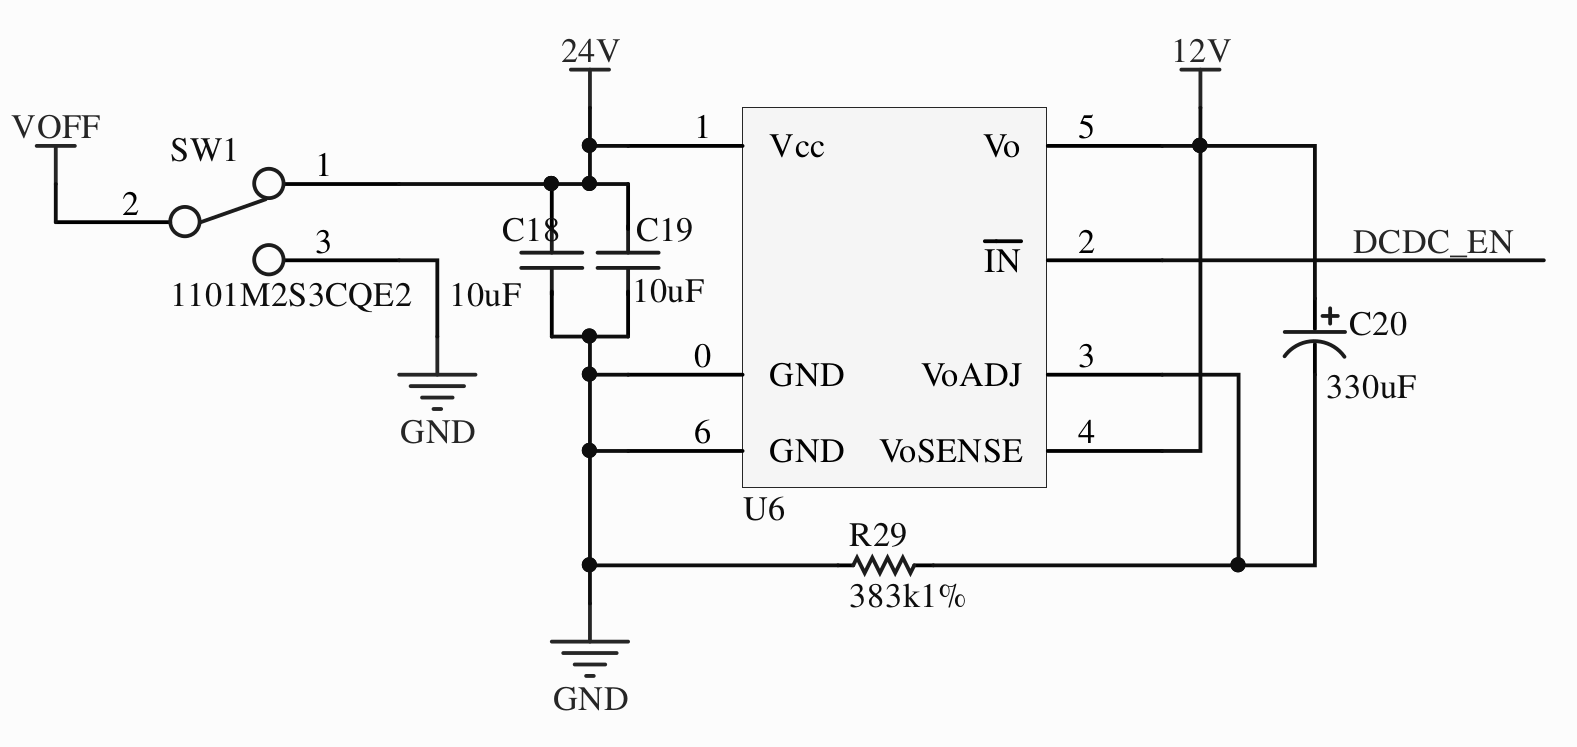
\includegraphics[width=\linewidth]{graphics/dcdc12v}
	\caption{The PTN78020H DC/DC converter and the appertaining circuitry.}
	\label{fig:dcdc12v}
\end{figure}

The \texttt{PTN78020H} DC/DC converter is used to generate the 12V rail. 
The component requires input and output capacitors in order to function properly and a resistor is needed to set the desired output voltage. 
The circuit used is based on the typical application circuit shown in the datasheet \cite{PTN78020H} and is implemented as shown in figure \ref{fig:dcdc12v}.
A resistor is required from \texttt{VoADJ} to ground to set the desired output voltage, in this case 12V.
In the datasheet on table 2 is a list of common voltages and the resistance required to achieve those voltages.
To generate 12V a 1\% 383 k$\Omega$ is needed.
\texttt{VoSENSE} should be connected close to the main load to allow for more precise regulation of the output.
This feature is mainly useful when the load is placed far from the supply and can be left floating if the accuracy of the rail is not important.
It was decided to simply short it to the 12V rail at the component since the load is placed relatively close to the supply.
$\overline{\text{\texttt{IN}}}$ carries the inhibit signal.
Pulling this low will disable the output of the component.
This is done by toggling the switch \texttt{SW1}. 
This will open a MOSFET which in turn will pull the \texttt{DCDC\_EN} signal low.
The datasheet also specifies that a ceramic capacitance of at least 18.8 $\mu$F is needed at the input. 
It was chosen to use two 10 $\mu$F capacitors.
In order to ensure stability the \texttt{PTN78020H} needs an output capacitance of 330 $\mu$F.
The datasheet specifies that if the application has load transients additional capacitance should be added to improve the response of the regulator.
While the load at the 12V rail is mostly steady, it does supply the boot capacitors which create a slight ripple on the rail.
It was therefore decided to use two 330 $\mu$F electrolytic capacitors in parallel.
As suggested by the datasheet an additional 20 $\mu$F of ceramic capacitance is added to the output to further improve the transient response.\\
\mikkel{Figure?}

\subsection{PTH08080W and LMR10510XMF} % (fold)
\label{sub:pth08080w}
As mentioned previously the choice of these component and the design of the circuitry around them was done by the authors in a previous project \cite{isaswarm} and the details of the design will be omitted for this discussion.
The PTH08080W and LMR10510XMF are responsible for creating the 5V and 3.3V rails, respectively.
These rails were designed mainly for ensuring the correct boot and shutdown of the MicroZed.
These procedures are described in detail in \cite{isaswarm}.
% subsection pth08080w (end)

\subsection{Motor Current Sensing}
\mikkel{A wild subsection appears! (Should be moved to a section where it makes sense)}
While reading in the literature it was found that measuring the current through the motor is beneficial for controlling the pendulums.
\thomas{This needs elaboration. Why is it beneficial? What does it add to the project?}

Current measurements are generally done by either hall effect based sensors or shunt resistors. 
Hall effect based sensors are usually better for high current applications where adding a resistor in series with the load is infeasible. 
Additionally, their interference with the circuit they are measuring is negligible.
Hall effect sensors do come at a higher cost and measuring smaller currents accurately may be a problem.
A shunt resistor used for current measurements is simply a resistor with a very low resistance, typically $<$ 100m$\Omega$, and a high power rating ranging from a few watts into 10's of watts depending on the application.
By adding such a resistor in series with the load, the voltage across the resistor can be measured and from that the current through the load determined.
This solution is simple and, if designed correctly, performs better at lower currents than hall effect sensors.
\thomas{source on performance of hall effect vs shunt resistors?}
This is beneficial since the current sensing in this project is used to do current mode control of the system, requiring a reasonably accurate measurement.
\thomas{What are the requirements of the accuracy? What can we achieve with the hardware?}
When measuring the current through an H-Bridge, as is done in this project, the shunt resistor can be placed in various positions.
The three main ones are high-side, in-line and low-side placement of the shunt resistor as shown in figure \ref{fig:shunt_measure_high_in_low}.

\begin{figure}[h]
	\centering
    %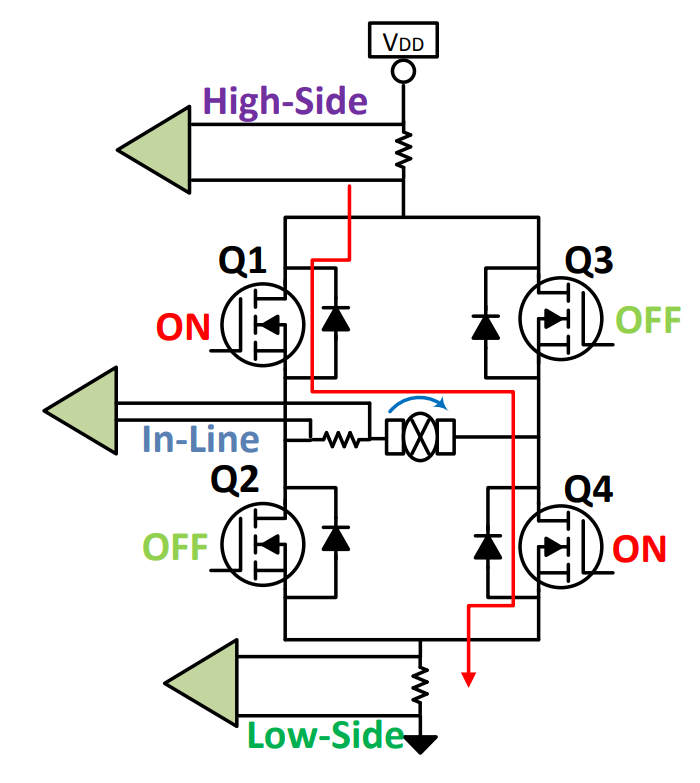
\includegraphics[width=0.5\linewidth]{graphics/shunt_sense_high_in_low}
	\caption{xxxx.}
	\label{fig:shunt_measure_high_in_low}
\end{figure}
\mikkel{Figure should be replaced by own illustration}

\cite{shunt_placement} and \cite{Current_Sense_Circuit_Collection} specifies the advantages and disadvantages of the three configurations.
\thomas{Perhaps add a quick summary of each and highlight the selected one?} 
Based on that it was decided to use the low-side configuration as it has low common voltage, it only needs a single sided supply and bi-directional current measurement is not needed.


\subsubsection{Requirements for the Current Measuring Circuit} % (fold)
\label{ssub:requirements_for_the_current_measuring_circuit}

The output of the current measuring circuit is an analogue signal that is measured by the ADC of the Zynq chip.
According to the Zynq ADC user guide \cite{zynq_adc}, the measurable input range is from 0V to 1V, but the maximum allowed input voltage is 1.9V according to \cite{adc_zynq_webanswer}.
The absolute maximum current through the motor is the stall current which is 80A, but the motor will run well below this level in normal operation.
The normal operation currents are expected to be up to 30A
\thomas{Some test or explanation required to justify 30A}
It was therefore decided that the circuit  needs to be able to measure currents of at least up to 40A.
The resolution per Ampere is increased by decreasing the current range that can be measured,
If the current gets any higher the ADC input should not be harmed meaning that the input voltage should not exceed 1.9V.

\mikkel{Below should be formatted differently}
\textbf{Requirements for the circuit:}
\begin{itemize}
	\item ADC input voltage does not exceed 1.9V when motor is stalling.
	\item Measures currents up to 40A, at minimum.
\end{itemize}

% subsubsection requirements_for_the_current_measuring_circuit (end)

\subsubsection{Designing the Current Measuring Circuit} % (fold)
\label{ssub:designing_the_current_measuring_circuit}

Placing a shunt resistor in the low-side configuration raises the voltage potential of the low-side of the H-bridge.
This may influence the gate signal required to open the MOSFETs of the H-bridge.
In addition, the shunt resistor will, regardless of placement result in a powerloss proportional to its size.
For these reasons minimizing the value of the shunt resistor is important. 
The smallest value available from the electronics supplier used at SDU provides a 200$\mu\Omega$ SMD shunt resistor.
Such a small resistance yields a minimal voltage drop and thus keeps power consumption at a minimum.\\
The resulting voltage from the motor stalling, that is an 80A current flowing through the resistor would result in only a 16mV voltage drop.
Since the input range of the ADC is 0-1V, this low voltage would yield very poor resolution in the area of actual interest, 0-40A.
An amplifier circuit is necessary.
Purpose built current-sense amplifiers exist which are used specifically for amplifying the voltage drop across a shunt resistor.
One such amplifier is the \texttt{INA286AID} from Texas Instruments \cite{INA286AID}.
It has a gain of 100, lifting the voltage resulting from motor stall to 1.6V as seen from \ref{eq:adc_input_voltage1} and \ref{eq:adc_input_voltage2}..
\begin{equation}
	V_{max,input} = G \cdot V_{shunt}
	\label{eq:adc_input_voltage1}
\end{equation}
\begin{equation}
	V_{max,input} = G \cdot R_{shunt} \cdot I_{stall} = 100 \cdot 200\cdot10^{-6} \cdot 80 = 1.6V
	\label{eq:adc_input_voltage2}
\end{equation}
The measurable range using this IC is 0-50A as seen from \ref{eq:adc_input_voltage3}.

\begin{equation}
	I_{max, measurable} = \frac{V_{max, measurable}}{R_{shunt}\cdot G} = \frac{1}{100 \cdot 200\cdot10^{-6} } = 50A
	\label{eq:adc_input_voltage3}
\end{equation}

\thomas{Is the information about 10mV full scale actually relevant to this design?}
and a very low offset allowing it to be used in applications where the maximum voltage drop across the shunt resistor is 10 mV full-scale 

This design meets the required design spec and the schematics can be seen in figure \ref{fig:currentmeasure}.
As can be seen, the INA286 in this configuration requires only the voltage input, \texttt{POWER\_SHUNT+/-} from the schematic on figure \ref{sfig:hbridgeshunt}, to generate a suitable output which is then fed directly to the ADC through the anti-aliasing filter shown on figure \ref{sfig:ina286aidschematic}.

\begin{figure}
	\centering
	\begin{subfigure}[b]{0.49\textwidth}
		\centering
		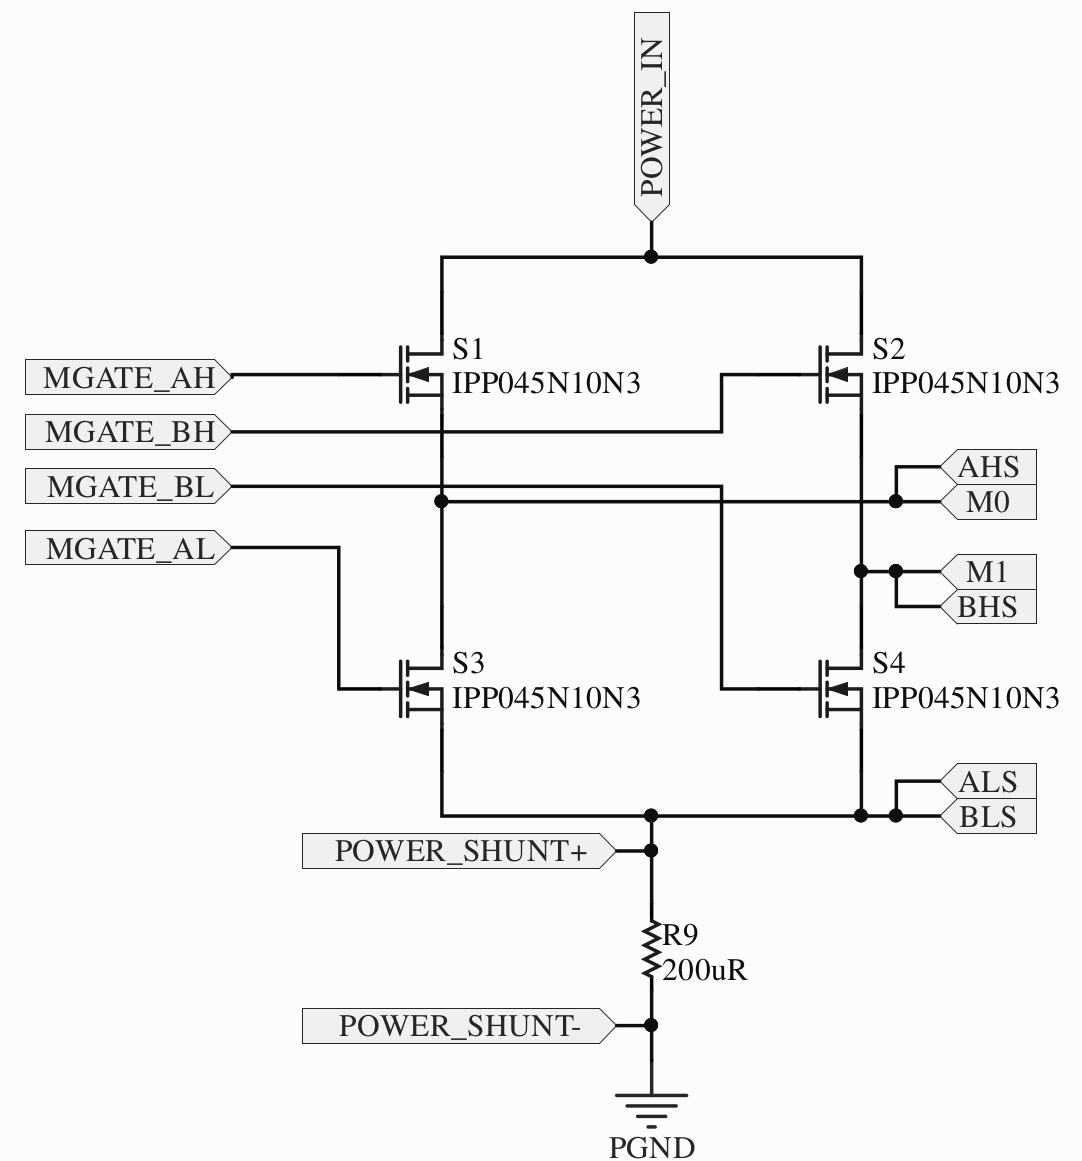
\includegraphics[width=\linewidth]{graphics/hbridge}
		\caption{H-bridge with shunt resistor in low-side configuration.}
		\label{sfig:hbridgeshunt}	
	\end{subfigure}
	\begin{subfigure}[b]{0.49\textwidth}
		\centering
		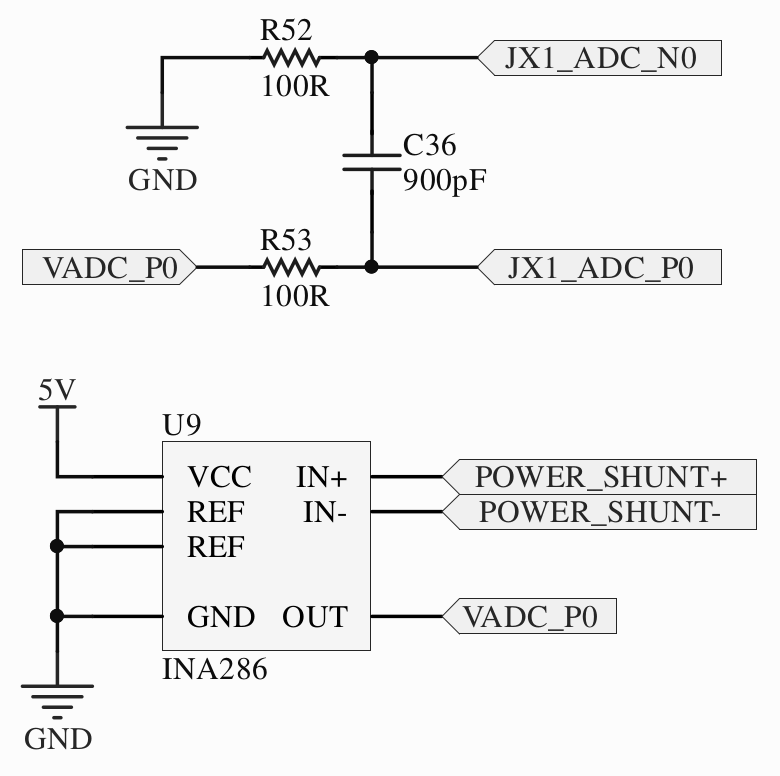
\includegraphics[width=\linewidth]{graphics/ina286}
		\caption{Schematic of the INA286AID as used in the project.}
		\label{sfig:ina286aidschematic}
	\end{subfigure}
	\caption{Schematics relating to the current measurement circuitry.}
	\label{fig:currentmeasure}
\end{figure}

% subsubsection designing_the_current_measuring_circuit (end)
\subsection{Relay Circuitry} % (fold)
\label{sub:relay_circuitry}

% subsection relay_circuitry (end)

\subsection{Endstop Detection} % (fold)
\label{sub:endstop_detection}
As described in section \ref{sub:safety_circuitry} it was decided to use infrared transceivers to detect endstops.
\mikkel{The actual 3D print design should be described elsewhere}
It was decided to use the \texttt{TCST 2103} as it has the wanted functionality.
It contains an infrared emitter pointing at a photo transistor, that conducts current proportional to the infrared light received.
In this project it will be used to detect if the infrared light rays has been blocked by the cart or not. 
The circuit shown in figure \ref{fig:tcst_circuit} was realised to convert the current conducted to a voltage level. 
The output is fed to a schmitt trigger circuit in order to be able to use the result as a boolean reference.
The schmitt trigger circuit is designed to have a high threshold of 3V and a low threshold of 1V. 

\begin{figure}
	\centering
	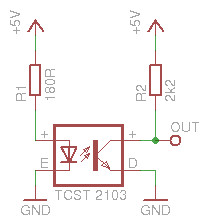
\includegraphics[width=0.4\linewidth]{graphics/tcst_circuit_temp.jpg}
	\caption{\texttt{TCST 2103} circuit.}
	\label{fig:tcst_circuit}
\end{figure}
\mikkel{replace with own image!}
% subsection endstop_detection (end)


% section board_design (end) 


\subsection{Schematic Revision} % (fold)
\label{sub:schematic_revision}

% subsection schematic_revision (end)
The authors experience with board design and layout ensures that a board layout is never error free in the first revision. 
This has been true even though a tremendous amount of work went into designing the board.
Therefore a strategy was devised to increase the likelihood of producing an error free board.
Many hours were spent on it, but hopefully it will relieve the authors of many hours of frustrating work on debugging the board and save money by removing the need of buying several different revisions of the PCB. 
The strategy consist of four steps that needs to be completed after finishing the design of the board:

\begin{itemize}
	\item Documentation
	\item General inspection
	\item Datasheet and report comparison
	\item Footprint inspection 
\end{itemize}

The content of each step will be elaborated here. 

\subsubsection*{Documentation}
Each circuit is documented to ensure that the design is done correctly.
Documenting a circuit requires studying the components datasheets and ensuring that they each meets the requirement.
Furthermore it requires a thorough inspection of the expected functionality of the circuit.
This step leads to correcting errors where a component is used wrong in respect to the wanted functionality of the circuit.

\subsubsection*{General Inspection}
General inspection of the schematic includes finding typographical errors on signals, components, resistor values, etc.
Furthermore each signal is inspected to ensure that it is connected correctly and it is also decided if it should be connected to an external header for measuring purposes.

\subsubsection*{Datasheet and Report Comparison}
Each circuit in the schematic is compared to its datasheets recommendation and the documentation written in the report. 
This step essentially ensures that each circuit has been verified more the one time. 
One could think that this step is irrelevant, but the authors believe it is important due to the complexity of the schematic.
After completion of this step, all circuits have been checked at least two times and the schematic a should be correct. 

\subsubsection*{Footprint Inspection}
Provided that the schematic is correct, the only possibly source of errors is the components footprints. 
Inspecting the footprint consist of verifying the correct pin assignment and the correct land patterns.
Both are done by inspecting each components datasheet. 
After completion of this step, both the schematic and footprints should be correct and the board is expected to be free from errors.
% section schematic_revision (end)